\documentclass{jfm}

% Compilation
\usepackage{silence} % Silence latex compiler warnings
\WarningFilter{latex}{Command \@xhline has changed} % Filter out warning
  % caused by redefinition between jfm.cls class and array (loaded by
  % siunitx)

% Import custom style file containing common packages and options
\setlength{\paperheight}{\pdfpageheight} % JFM class removes paperheight definition and hyperref raises a warning

% Import custom style file containing common packages and options
\usepackage{preamble}
\graphicspath{{./Figures/}}

% Discrete Fourier Transform
\newcommand{\GenP}{\hat{P}_m}
\newcommand{\POne}{\hat{P}_1}
\newcommand{\PTwo}{\hat{P}_2}
\newcommand{\PThree}{\hat{P}_3}
\newcommand{\PFour}{\hat{P}_4}

% Continuous Fourier Transform
\newcommand{\GenPk}{\hat{P}(\kappa)}
\newcommand{\PZerok}{\hat{P}(0)}

% Define custom math symbols
\DeclareMathOperator{\cn}{Cn}
\DeclareMathOperator{\sgn}{sgn}
\DeclareMathOperator{\Ur}{Ur}
\DeclareMathOperator{\Sk}{Sk}
\DeclareMathOperator{\As}{As}
%\DeclareMathOperator{\Bi}{Bi}

% Define \im as Roman i
\newcommand{\im}{\mathrm{i}}
% Replace epsilon with varepsilon
\renewcommand*{\epsilon}{\varepsilon}

%% Use \thalf and \squart commands from JFM class
%\newcommand\squart{\ensuremath{{\textstyle\frac{1}{4}}}}
%\newcommand\thalf{\ensuremath{{\textstyle\frac{1}{2}}}}

\linenumbers

\title{Wind-Induced Changes to Surface Gravity Wave Shape in Shallow Water}

\author{Thomas J. Zdyrski \and Falk Feddersen}

\begin{document}

\begin{figure}
  \centering
  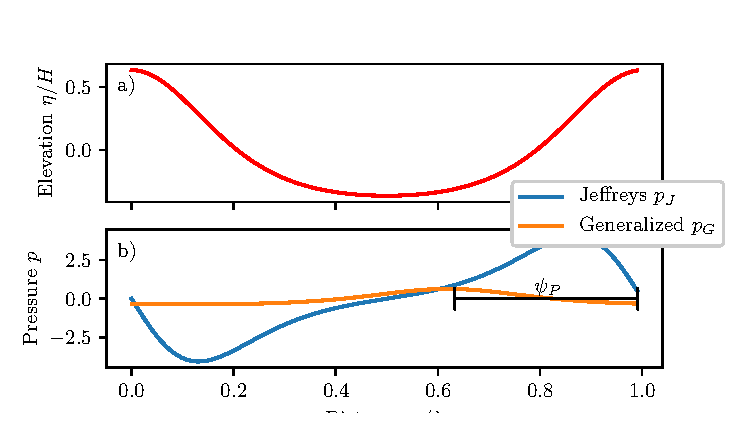
\includegraphics{Forcing-Types.eps}
  \caption{
    Forcing types with normalized nondimensional pressure P as a
    function of nondimensional distance $x/\lambda$.
  }
\end{figure}

\begin{figure}
  \centering
  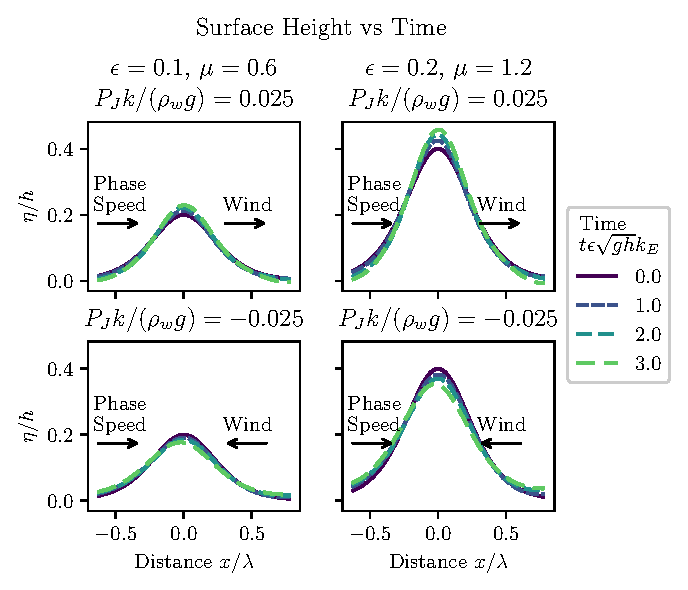
\includegraphics{Snapshots-Positive-Negative.eps}
  \caption{
    Evolution of a solitary wave profile under onshore and offshore Jeffreys
    forcing.
  }
\end{figure}

\begin{figure}
  \centering
  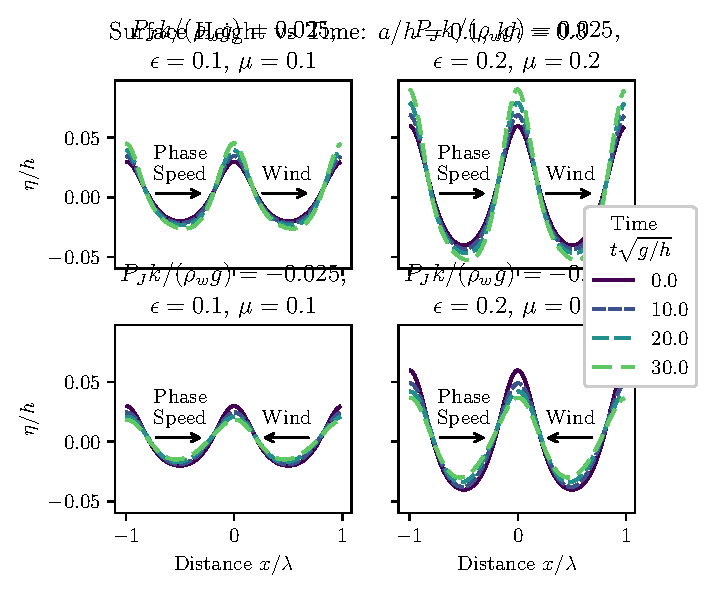
\includegraphics{Snapshots-Positive-Negative-Cnoidal.eps}
  \caption{
    Evolution of a cnoidal profile under onshore and offshore Jeffreys
    forcing.
  }
\end{figure}

\begin{figure}
  \centering
  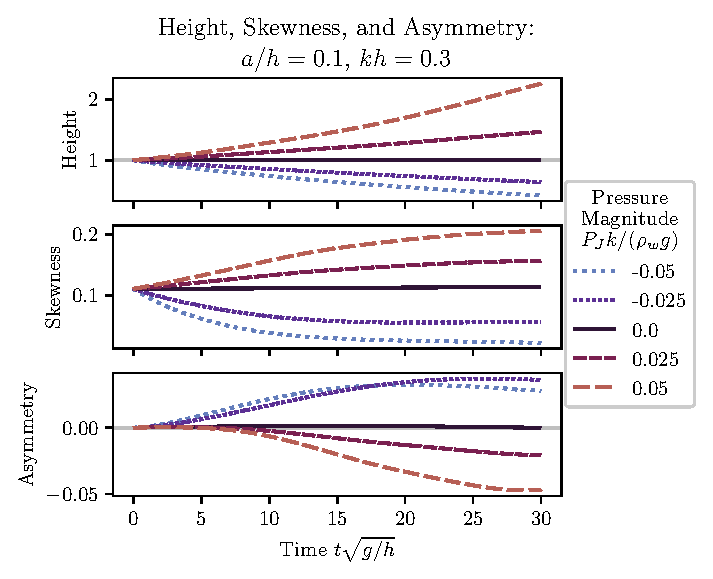
\includegraphics{Skew-Asymm-Cnoidal.eps}
  \caption{
    Skewness and asymmetry of cnoidal profile under onshore and offshore
    Jeffreys forcing.
  }
\end{figure}

\begin{figure}
  \centering
  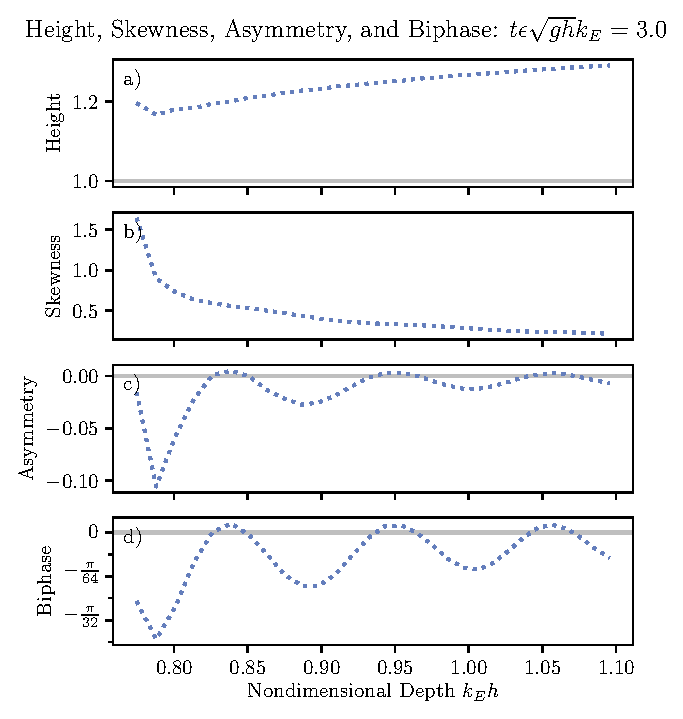
\includegraphics{Skew-Asymm-Cnoidal-kh.eps}
  \caption{
    Skewness and asymmetry of cnoidal profile under onshore forcing as a
    function of nondimensional depth $kh$.
  }
\end{figure}

\begin{figure}
  \centering
  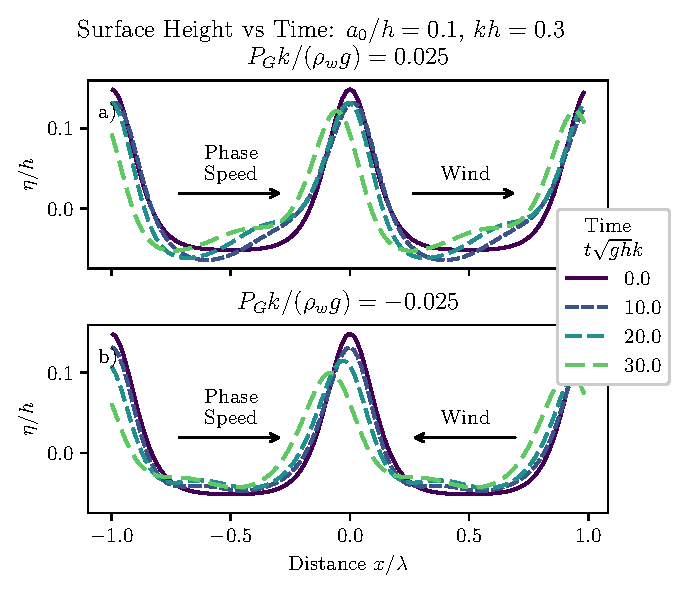
\includegraphics{Snapshots-Positive-Negative-Cnoidal-GM.eps}
  \caption{
    Evolution of a cnoidal profile under onshore and offshore Generalized
    Miles forcing.
  }
\end{figure}

\begin{figure}
  \centering
  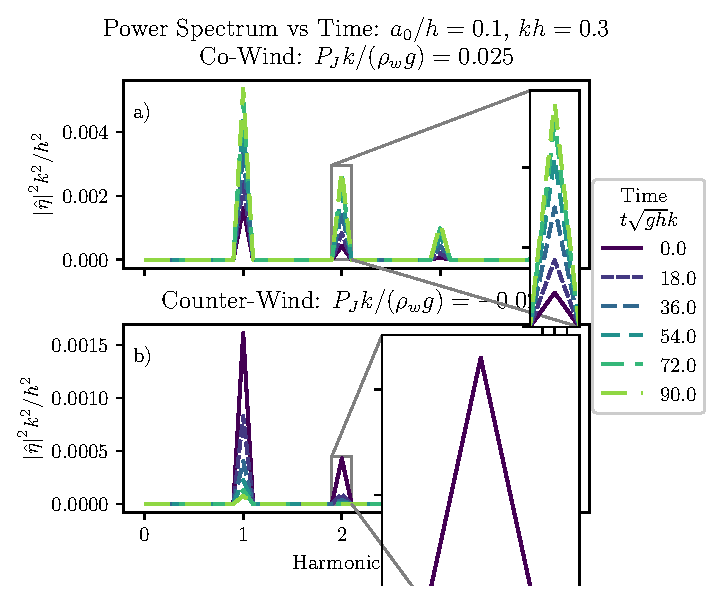
\includegraphics{Power-Spectrum-Jeffreys.eps}
  \caption{
    Power spectrum of cnoidal wave under Jeffreys forcing.
  }
\end{figure}

\begin{figure}
  \centering
  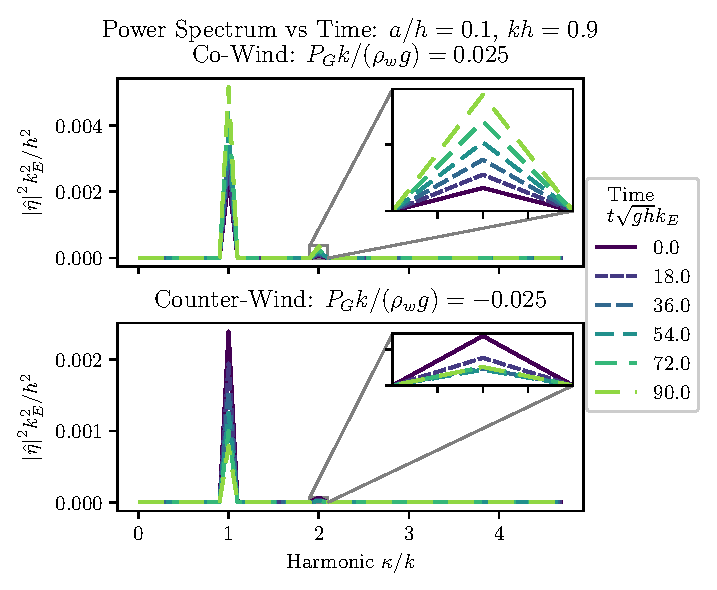
\includegraphics{Power-Spectrum-GM.eps}
  \caption{
    Power spectrum of cnoidal wave under Generalized Miles forcing.
  }
\end{figure}

\begin{figure}
  \centering
  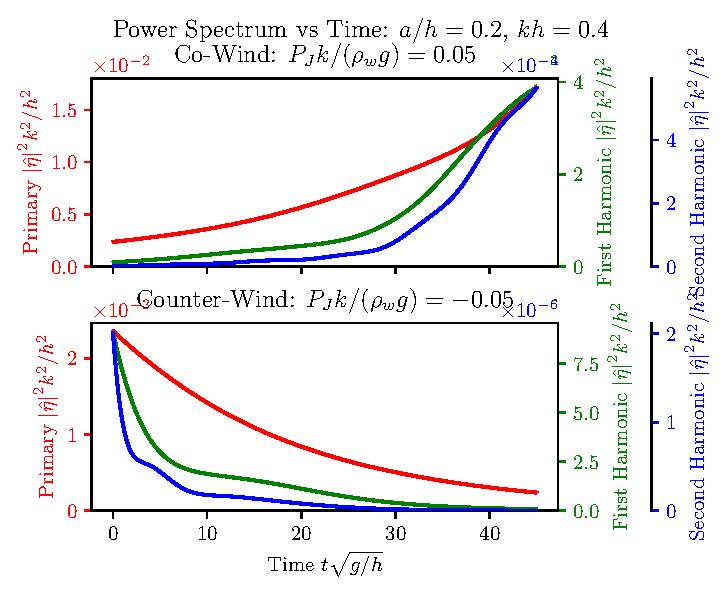
\includegraphics{Power-Spectrum-vs-Time-Jeffreys.eps}
  \caption{
    Power spectrum of cnoidal wave under Jeffreys forcing as a function
    of time.
  }
\end{figure}

\begin{figure}
  \centering
  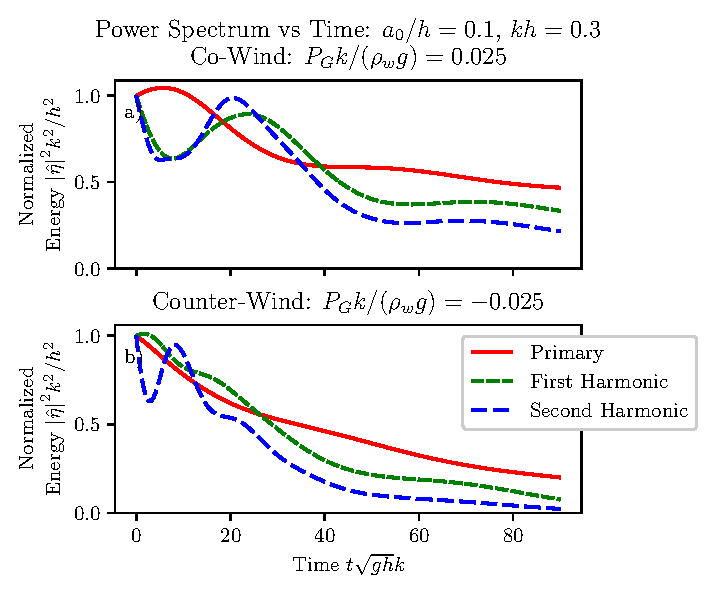
\includegraphics{Power-Spectrum-vs-Time-GM.eps}
  \caption{
    Power spectrum of cnoidal wave under Generalized Miles forcing as a
    function of time.
  }
\end{figure}

\end{document}
